\documentclass{article}
\usepackage[a4paper,top=0.6in, bottom=0.5in, left=1in, right=1in,footskip=0.1in]{geometry}
%\usepackage{fullpage}
\usepackage{listings}
\usepackage{gensymb}
\usepackage{hyperref}
\hypersetup{
	 colorlinks   = true,
     citecolor    = black,
     linkcolor    = black,
     urlcolor     = black
}
\usepackage{graphicx}
\usepackage{algorithm}
\usepackage{algpseudocode}
\usepackage{amsmath}
\usepackage{amssymb}
\usepackage{tikz}
\usepackage{caption}
\usepackage{subcaption}
\usepackage{float}
\usetikzlibrary{arrows,matrix,positioning}
\setcounter{tocdepth}{3}
\begin{document}
\title{DIP Homework 4}
\author{Qiuyi Zhang 12330402 \\ \href{mailto:joyeec9h3@gmail.com}{joyeec9h3@gmail.com}} 
\date{\today}
\maketitle
\tableofcontents
\section{Exercises}

\subsection{Color Spaces}

\textbf{Answer:} 

\begin{enumerate}
\item Advantages of HSI color space:
\begin{enumerate}
\item xxx
\item xxx
\end{enumerate}

\item Adding $120\degree$ to the Hue components
\end{enumerate}

\subsection{Color Composition}

\textbf{Answer:}

General expression


% -------------------- Programming Tasks ------------------------
\section{Programming Tasks}
% -------------------- Fourier Transform ------------------------
\subsection{Image Filtering}
% -------------------- Results ------------------------

\begin{figure}[H]
	\centering
	% pt = px * 72 / DPI
	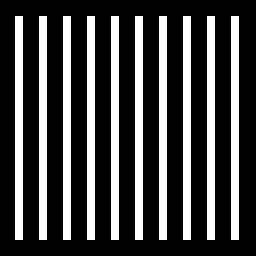
\includegraphics[width=192pt]{../img/task_1.png}
	\caption{The original image}
\end{figure}

\subsubsection{Arithmetic mean filter}

The images filtered with $3 \times 3$ and $9 \times 9$ arithmetic mean filters are shown in Figure~\ref{fig:baram33} and~\ref{fig:baram99}.

Both filters make the bars appear to be ``smaller'' in both height and width. Since the white sides of the edges will take the mean of their neighborhood as their new intensities, they will be grey instead of white after filtering, thus visually ``shrinking'' the bars. This effect also darkens the overall color of the image.

\begin{figure}[H]
	\captionsetup{justification=centering,margin=1cm}
	\begin{minipage}[b]{0.48\linewidth}
		\centering
		% pt = px * 72 / DPI
		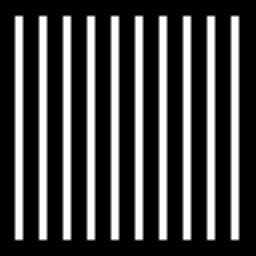
\includegraphics[width=192pt]{../result/task1/arithmetic-mean-3-3.png}
		\caption{Filtered with $3 \times 3$ arithmetic mean filter}
		\label{fig:baram33}
	\end{minipage}
	\begin{minipage}[b]{0.48\linewidth}
		\centering
		% pt = px * 72 / DPI
		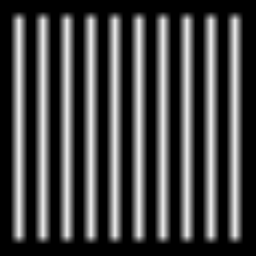
\includegraphics[width=192pt]{../result/task1/arithmetic-mean-9-9.png}
		\caption{Filtered with $9 \times 9$ arithmetic mean filter}
		\label{fig:baram99}
	\end{minipage}
\end{figure}


\subsubsection{Harmonic mean filter}

The images filtered with $3 \times 3$ and $9 \times 9$ harmonic mean filters are shown in Figure~\ref{fig:barhm33} and~\ref{fig:barhm99}.

The expression of harmonic mean filtering is:

$$
\hat{f}(x, y) = \frac{mn}{\sum_{(s, t)\in S_{xy}} \frac{1}{g(s, t)}}
$$

Once there is any $g(s, t) = 0$, then $\sum_{(s, t)\in S_{xy}} \frac{1}{g(s, t)} = \infty$, then $\hat{f}(x, y) = 0$. Assuming $n$ is odd, $n = 2k + 1$ and $2k <$ the distance between the bars, an $n \times n$ harmonic mean filter will ``blacken'' $k$ pixels of the edges of the bars in every direction. Therefore with a $3 \times 3$ harmonic filter, the bars are $2 \times 1 = 2$ pixels thiner, $2 \times 1 = 2$ pixels shorter. When the neighborhood is $9 \times 9$, the bars are $4 \times 1 = 4$ pixels thiner, $4 \times 1 = 4$ pixels shorter, which effectively makes the bars disappear.


\begin{figure}[H]
	\captionsetup{justification=centering,margin=1cm}
	\begin{minipage}[b]{0.48\linewidth}
		\centering
		% pt = px * 72 / DPI
		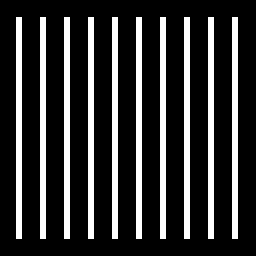
\includegraphics[width=192pt]{../result/task1/harmonic-mean-3-3.png}
		\caption{Filtered with $3 \times 3$ harmonic mean filter}
		\label{fig:barhm33}
	\end{minipage}
	\begin{minipage}[b]{0.48\linewidth}
		\centering
		% pt = px * 72 / DPI
		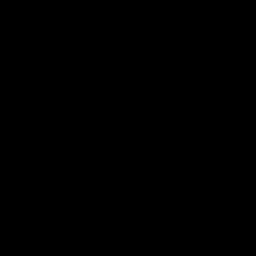
\includegraphics[width=192pt]{../result/task1/harmonic-mean-9-9.png}
		\caption{Filtered with $9 \times 9$ harmonic mean filter}
		\label{fig:barhm99}
	\end{minipage}
\end{figure}

\subsubsection{Contraharmonic mean filter}

The images filtered with $3 \times 3$ and $9 \times 9$ contraharmonic mean filters are shown in Figure~\ref{fig:barchm33} and~\ref{fig:barchm99}

The expression of contraharmonic mean filtering is:

$$
\hat{f}(x, y) = \frac{\sum_{(s, t)\in S_{xy}} g(s, t)^{Q+1}}{\sum_{(s, t)\in S_{xy}} g(s, t)^Q}
$$

When $Q < 0$, once there is any $g(s, t) = 0$, then $\sum_{(s, t)\in S_{xy}} g(s, t)^{Q} = 0$, then $\hat{f}(x, y) = 0$. When $Q = -1.5$, using the same reasoning as for the harmonic mean filter, a $3 \times 3$ contraharmonic filter will make the bars $2 \times 1 = 2$ pixels thiner, $2 \times 1 = 2$ pixels shorter. A $9 \times 9$ contraharmonic filter will make the bars $4 \times 1 = 4$ pixels thiner, $4 \times 1 = 4$ pixels shorter, effectively making the bars disappear.

\begin{figure}[H]
	\captionsetup{justification=centering,margin=0.5cm}
	\begin{minipage}[b]{0.48\linewidth}
		\centering
		% pt = px * 72 / DPI
		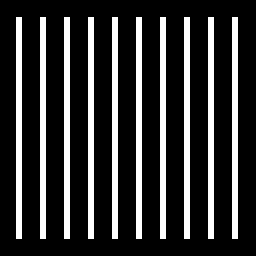
\includegraphics[width=192pt]{../result/task1/contraharmonic-mean-3-3.png}
		\caption{Filtered with $3 \times 3$ contraharmonic mean filter($Q=-1.5$)}
		\label{fig:barchm33}
	\end{minipage}
	\begin{minipage}[b]{0.48\linewidth}
		\centering
		% pt = px * 72 / DPI
		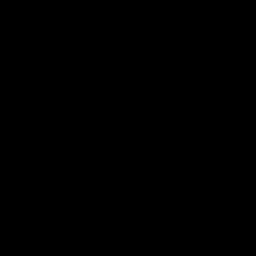
\includegraphics[width=192pt]{../result/task1/contraharmonic-mean-9-9.png}
		\caption{Filtered with $9 \times 9$ contraharmonic mean filter($Q=-1.5$)}
		\label{fig:barchm99}
	\end{minipage}
\end{figure}

% End results and descirptions


\subsection{Image Denoising}

\subsubsection{Statistical filters}

\paragraph{Algorithm}
\begin{algorithm}
\centering
\caption{Statistical filters}
\label{alg:statfilt}
  \begin{algorithmic}[1]
    \Function{stat\_filter}{$input\_img$, $size$, $p$}
        \Comment{$input\_img$ is the input image}
        \State $output\_img = $ a new image \Comment{$size$ is the size of the neighborhood} 
	    \For{each pixel $(x, y)$ in $input\_img$} \Comment{$p$ is the percentile}
    		\State Get the neighborhood of $(x, y)$
    		\State Get the $p_{th}$ percentile in the neighborhood
    		\State Put the $p_{th}$ percentile to the pixel $(x, y)$ in $output\_image$
	    \EndFor
      \State \Return $output\_image$
    \EndFunction
\\
    \Function{max\_filter}{$input\_img$, $size$}
    	\State \Return \Call{stat\_filter}{$input\_img$, $size$, $100$}
    \EndFunction
\\
    \Function{min\_filter}{$input\_img$, $size$}
    	\State \Return \Call{stat\_filter}{$input\_img$, $size$, $0$}
    \EndFunction
\\
    \Function{median\_filter}{$input\_img$, $size$}
    	\State \Return \Call{stat\_filter}{$input\_img$, $size$, $50$}
    \EndFunction
  \end{algorithmic}
\end{algorithm}

\begin{figure}[]
	\centering
	% pt = px * 72 / DPI
	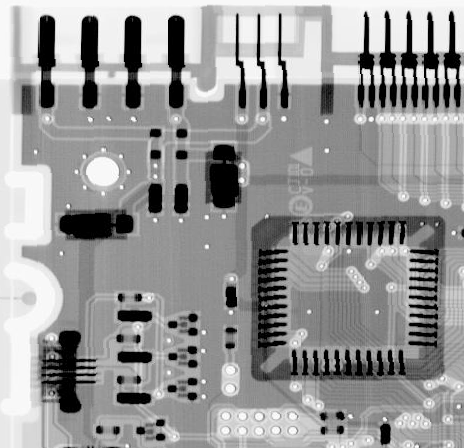
\includegraphics[width=336pt]{../img/task_2.png}
	\caption{The original image}
\end{figure}

\subsubsection{Gaussian noise and denoising}

\begin{figure}[]
	\centering
	% pt = px * 72 / DPI
	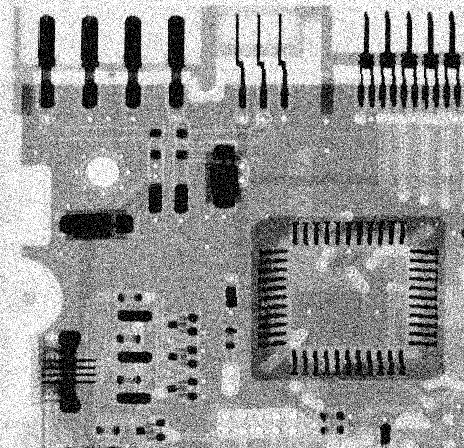
\includegraphics[width=336pt]{../result/task2/gauss/gauss-0-40.png}
	\caption{Image with gaussian noise($\mu = 0, \sigma = 40$)}
	\label{fig:gauss}
\end{figure}

\begin{figure}[]
	\centering
	% pt = px * 72 / DPI
	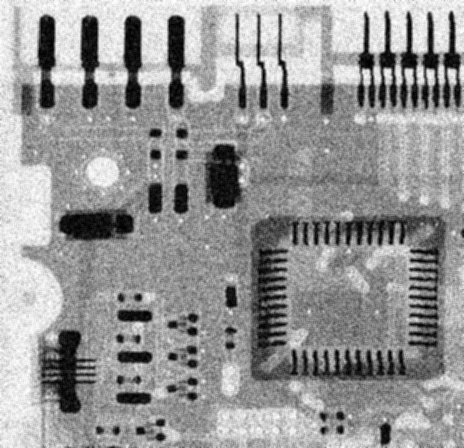
\includegraphics[width=336pt]{../result/task2/gauss/gauss-arithmetic.png}
	\caption{Gaussian noise filtered with $3 \times 3$ arithmetic mean filter}
	\label{fig:gaussam}
\end{figure}

\begin{figure}[]
	\centering
	% pt = px * 72 / DPI
	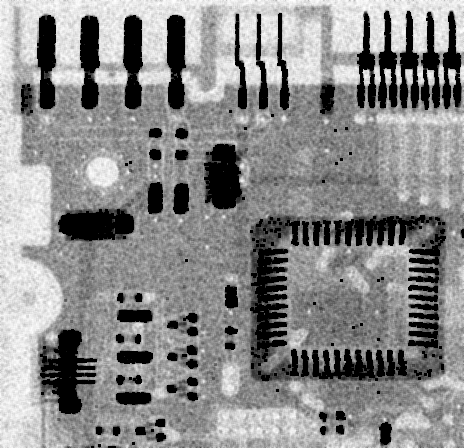
\includegraphics[width=336pt]{../result/task2/gauss/gauss-geometric.png}
	\caption{Gaussian noise filtered with $3 \times 3$ geometric mean filter}
	\label{fig:gaussgm}
\end{figure}

\begin{figure}[]
	\centering
	% pt = px * 72 / DPI
	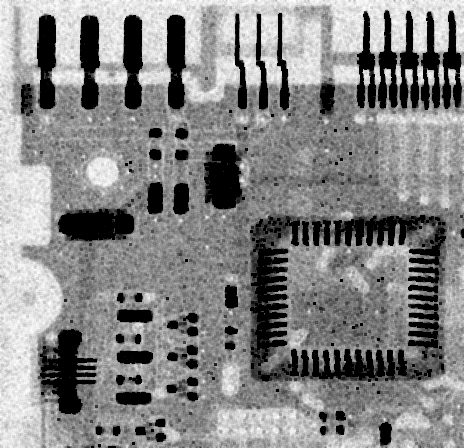
\includegraphics[width=336pt]{../result/task2/gauss/gauss-harmonic.png}
	\caption{Gaussian noise filtered with $3 \times 3$ harmonic mean filter}
	\label{fig:gausshm}
\end{figure}

\begin{figure}[]
	\centering
	% pt = px * 72 / DPI
	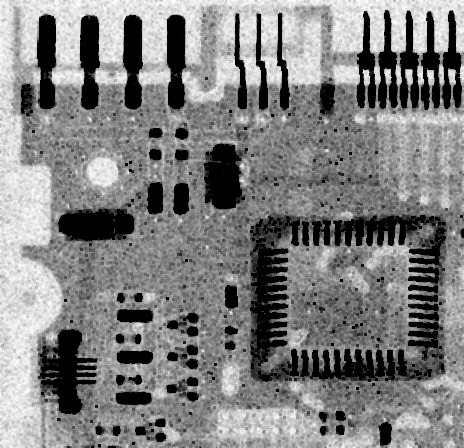
\includegraphics[width=336pt]{../result/task2/gauss/gauss-contraharmonic.png}
	\caption{Gaussian noise filtered with $3 \times 3$ contraharmonic mean filter($Q = -1.5$)}
	\label{fig:gausschm}
\end{figure}

\begin{figure}[]
	\centering
	% pt = px * 72 / DPI
	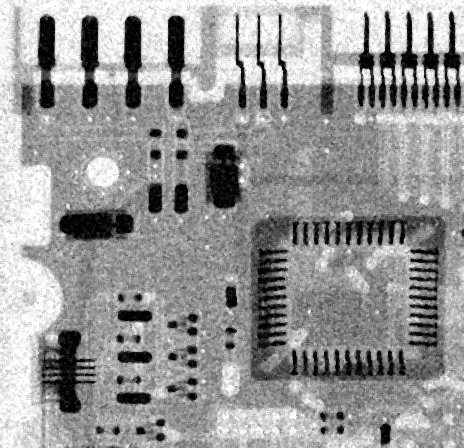
\includegraphics[width=336pt]{../result/task2/gauss/gauss-median.png}
	\caption{Gaussian noise filtered with $3 \times 3$ median filter}
	\label{fig:gaussm}
\end{figure}


\paragraph{Discussion}
Both arithmetic mean filtering (Figure~\ref{fig:gaussam}) and geometric mean filtering (Figure~\ref{fig:gaussgm}) successully reduce the noise in the image. Since the geometric mean is more suitable for drastically different terms by nature, the geometric mean filter can better preserve the edges in the image. Therefore it does not blur the image as much as the arithmetic mean filter. Nonetheless, since any pixel in the neighborhood with intensity $0$ would make the geometric mean $0$, there are some unpleasent black flakes scattered in the image denoised with geometric mean filter.

As explained in the analysis of filtered bar images, the harmonic mean filter (Figure~\ref{fig:gausshm}) and the contraharmonic filter (Figure~\ref{fig:gausschm}) have the same problem as the geometric mean filter -- unpleasent black flakes. They both reduces some noise, but not as good as the arithmetic mean filter and the geometric mean filter.

The median filter (Figure~\ref{fig:gaussm}) does the best job at denoising the image since it's very suitable for random noise like this. It also has considerably less
blurring than the others.

\subsubsection[H]{Salt noise and denoising}


\begin{figure}[H]
	\centering
	% pt = px * 72 / DPI
	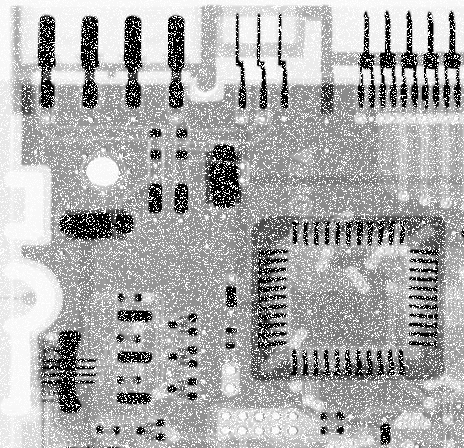
\includegraphics[width=336pt]{../result/task2/salt/salt-20.png}
	\caption{Image with salt noise($p=0.2$)}
	\label{fig:salt}
\end{figure}

\begin{figure}[H]
	\centering
	% pt = px * 72 / DPI
	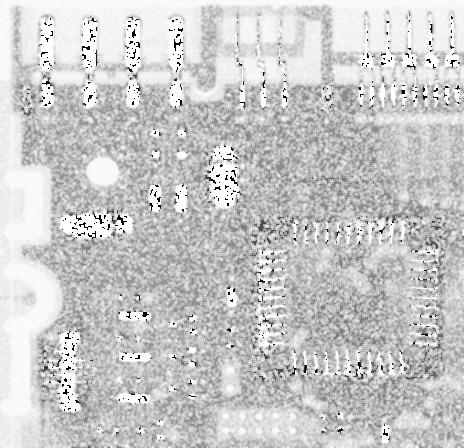
\includegraphics[width=336pt]{../result/task2/salt/salt-contraharmonic-1-5.png}
	\caption{Salt noise filtered with $3 \times 3$ contraharmonic mean filter($Q = 1.5$)}
	\label{fig:saltchmpos}
\end{figure}

\begin{figure}[H]
	\centering
	% pt = px * 72 / DPI
	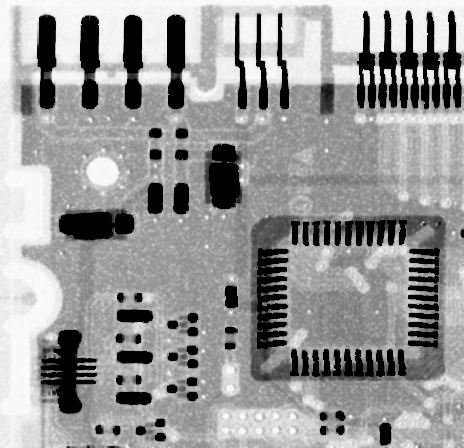
\includegraphics[width=336pt]{../result/task2/salt/salt-contraharmonic--1-5.png}
	\caption{Salt noise filtered with $3 \times 3$ contraharmonic mean filter($Q = -1.5$)}
	\label{fig:saltchmneg}
\end{figure}

\paragraph{Discussion}
The expression of contraharmonic mean filtering is:

$$
\hat{f}(x, y) = \frac{\sum_{(s, t)\in S_{xy}} g(s, t)^{Q+1}}{\sum_{(s, t)\in S_{xy}} g(s, t)^Q}
$$

When salt noise is added to the image, the noise value is relatively large. Consider a $3 \times 3$ neighborhood with the noise $intensity = 255$ as its center and others $intensity = 0$. when $Q < 0$, the small numbers in the neighborhood will dominate the result. The numerator can then be thought of as a constant raised to $Q + 1$ and the denominator as a the same constant raised to $Q$. This constant is then the value of the pixels in the neighborhood. So the ratio is just that value. Therefore, a $Q < 0$ can effectively reduce the salt noise in the image. But when $Q > 0$, the large center will dominate the contraharmonic mean, and affect the pixels around it. In this case, other pixels will be incorrectly lightened, making the image look worse.

\subsubsection{Salt-and-pepper noise and denoising}
\paragraph{Results}


\begin{figure}[H]
	\centering
	% pt = px * 72 / DPI
	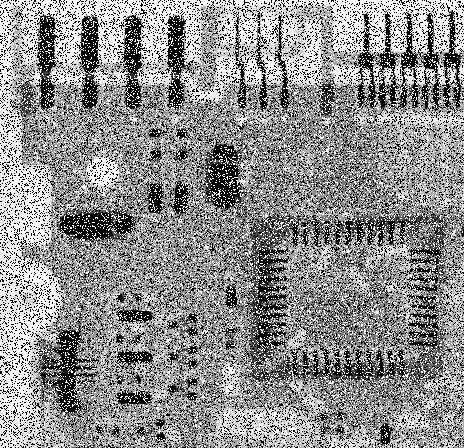
\includegraphics[width=336pt]{../result/task2/sap/sap-20-20.png}
	\caption{Image with salt noise($p=0.2$) and pepper noise($p=0.2$)}
	\label{fig:sap}
\end{figure}

\begin{figure}[H]
	\centering
	% pt = px * 72 / DPI
	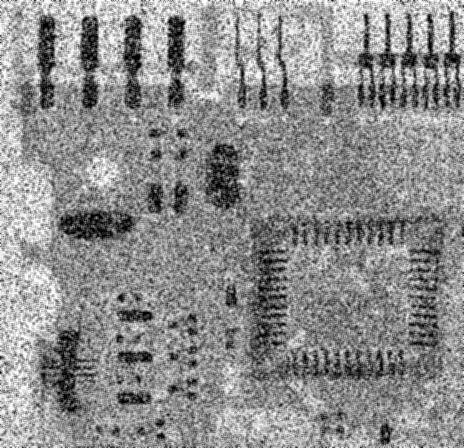
\includegraphics[width=336pt]{../result/task2/sap/sap-arithmetic.png}
	\caption{Salt-and-pepper noise filtered with $3 \times 3$ arithmetic mean filter}
	\label{fig:sapam}
\end{figure}

\begin{figure}[H]
	\centering
	% pt = px * 72 / DPI
	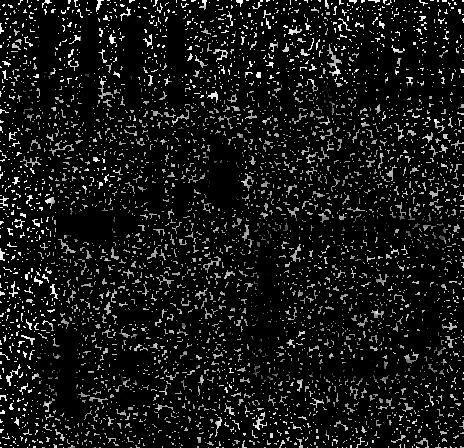
\includegraphics[width=336pt]{../result/task2/sap/sap-harmonic.png}
	\caption{Salt-and-pepper filtered with $3 \times 3$ harmonic mean filter}
	\label{fig:saphm}
\end{figure}


\begin{figure}[H]
	\centering
	% pt = px * 72 / DPI
	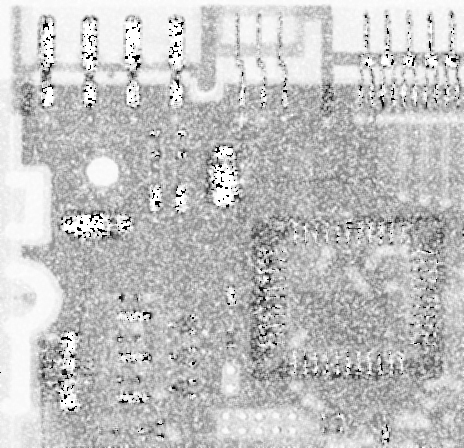
\includegraphics[width=336pt]{../result/task2/sap/sap-contraharmonic.png}
	\caption{Salt-and-pepper noise filtered with $3 \times 3$ contraharmonic mean filter($Q=0.5$)}
	\label{fig:sapchm}
\end{figure}

\begin{figure}[H]
	\centering
	% pt = px * 72 / DPI
	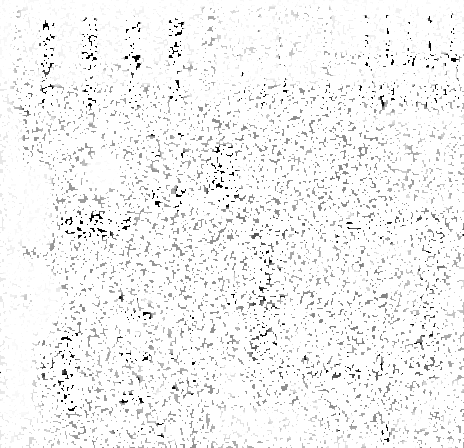
\includegraphics[width=336pt]{../result/task2/sap/sap-max.png}
	\caption{Salt-and-pepper noise filtered with $3 \times 3$ max filter}
	\label{fig:sapmax}
\end{figure}

\begin{figure}[H]
	\centering
	% pt = px * 72 / DPI
	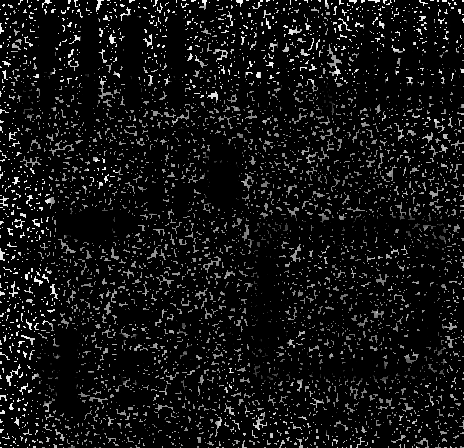
\includegraphics[width=336pt]{../result/task2/sap/sap-min.png}
	\caption{Salt-and-pepper noise filtered with $3 \times 3$ min filter}
	\label{fig:sapmin}
\end{figure}

\begin{figure}[H]
	\centering
	% pt = px * 72 / DPI
	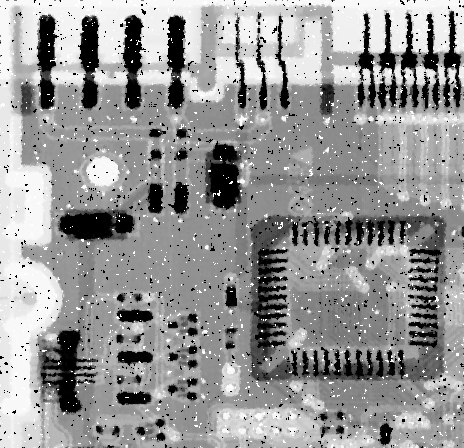
\includegraphics[width=336pt]{../result/task2/sap/sap-median.png}
	\caption{Salt-and-pepper noise filtered with $3 \times 3$ median filter}
	\label{fig:sapmedian}
\end{figure}

\paragraph{Discussion}

When there are both salt noise with $p = 0.2$ and pepper noise with $p = 0.2$ in the image, for a $3 \times 3$ neighborhood, the expected number of pixels with $intensity = 0$ is $9 \times 0.2 = 1.8$, same as the expected number of pixels with $intensity = L - 1$. Therefore in a $3 \times 3$ neighborhood there are likely $1 ~ 2$ pixels with the minimum intensity and $1 ~ 2 pixels$ with the minimun intensity.

The arithmetic mean filter reduces some noises (as shown in Figure~\ref{fig:sapam}), making the objects in the image more recognizable, but there are still a considerable amount of noises in the result. Because of the indensity (approximately $40\%$) and the extreme values of the noises, it is hard for an arithmetic mean filter to produce a satisfying result.

As explained in previous sections, once there is any pixels with $intensity = 0$ in the neighborhood, the output of a harmonic mean filter will be $0$ too. Since we expect more than $1$ pixel with $intensity = 0$ in any $3 \times 3$ neighborhood, most pixels of the filtered image will be turned black, leading to terrible results, as shown in Figure~\ref{fig:saphm}.

Since a contraharmonic mean filter can only handle salt noise \textbf{or} pepper noise but not both at the same time, in this case, it makes the result look worse, as shown in Figure~\ref{fig:sapchm}.

Because we expect more than $1$ pixel with the minimun intensity and more than $1$ pixel with the maximun intensity in any $3 \times 3$ neighborhood, most pixels in the result of a max filter will have the maximun intensity and a minimun filter minimun intensity. Both results are disastrous, as shown in Figure~\ref{fig:sapmax} and~\ref{fig:sapmin}.

Although the median filter successfully restores most of the image, because of the high indensity of the noise, there are still some visible noises in the result, as shown in Figure~\ref{fig:sapmedian}.

\subsection{Histogram Equalization on Color Images}

\subsubsection{Results}

\begin{figure}[H]
	\centering
	% pt = px * 72 / DPI
	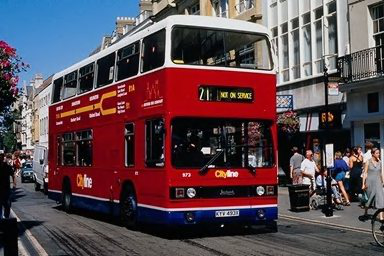
\includegraphics[width=288pt]{../img/02.png}
	\caption{The original image}
\end{figure}

\begin{figure}[H]
	\centering
	% pt = px * 72 / DPI
	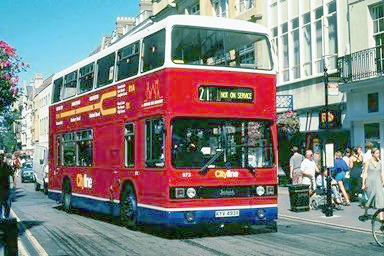
\includegraphics[width=288pt]{../result/hist/hist-seperate.png}
	\caption{Image rebuilt with three channels equalized with different histograms}
\end{figure}

\begin{figure}[h]
	\centering
	% pt = px * 72 / DPI
	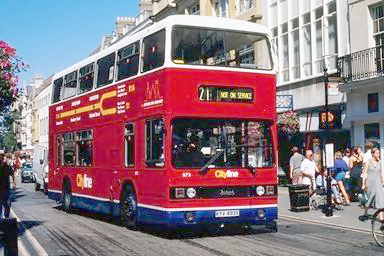
\includegraphics[width=288pt]{../result/hist/hist-together.png}
	\caption{Image rebuilt with three channels equalized with the same average histogram}
\end{figure}


\end{document}